% 2D Vector Addition
%
% File:         2d-vector-addition.tex
% Author:       Bob Walton (walton@acm.org)
% Date:      	Thu Dec 20 18:24:26 EST 2012
  
\documentclass{minimal}
\usepackage[paperheight=3in,paperwidth=2in,
            height=3in,hoffset=0.05in,
	    voffset=0.05in,left=0in,width=2in]{geometry}
\usepackage{color}
\usepackage[usenames]{xcolor}
\usepackage{scalefnt}
\usepackage{tikz}
\newcommand{\SMALL}{\scalefont{0.8}}
\usetikzlibrary{arrows}
\begin{document}
\raggedright
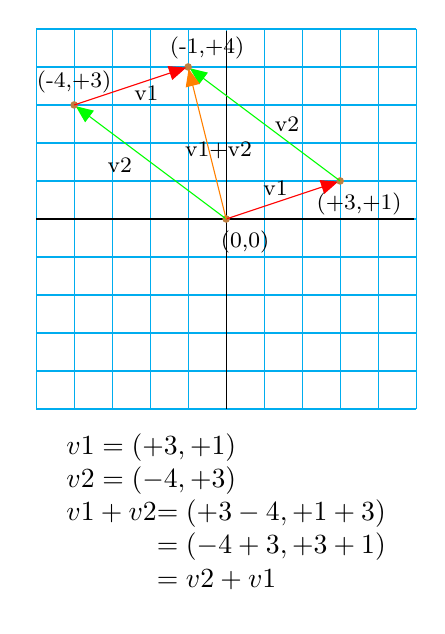
\begin{tikzpicture}[x=0.190in,y=0.190in]
\begin{scope}[yshift=1in,>=triangle 45,shorten >=0.01in]
    \draw[cyan] (-5,-5) grid[step=1] (5,5);
    \draw[black] (-5,0) -- (+5,0);
    \draw[black] (0,-5) -- (0,+5);

    \fill[brown] (0,0) circle(0.1) + (+0.5,-0.6) node[black]{\SMALL (0,0)};

    \draw[red,->] (0,0) -- (+3,+1);
    \draw[black] (1.3,0.8) node{\SMALL v1};
    \fill[brown] (+3,+1) circle(0.1) + (+0.5,-0.6) node[black]{\SMALL (+3,+1)};
    \draw[green,->] (+3,+1) -- (-1,+4);
    \draw[black] (+1.6,2.5) node{\SMALL v2};
    \fill[brown] (-1,+4) circle(0.1) + (+0.5,+0.5) node[black]{\SMALL (-1,+4)};

    \draw[green,->] (0,0) -- (-4,+3);
    \draw[black] (-2.8,1.4) node{\SMALL v2};
    \fill[brown] (-4,+3) circle(0.1) + (+0.0,+0.6) node[black]{\SMALL (-4,+3)};
    \draw[red,->] (-4,+3) -- (-1,+4);
    \draw[black] (-2.1,3.3) node{\SMALL v1};

    \draw[orange,->] (0,0) -- (-1,+4);
    \draw[black] (-0.2,1.8) node{\SMALL v1+v2};
\end{scope}

\begin{scope}
\draw (0,-2.5) node {
    $\begin{array}{l}
    v1 = (+3,+1) \\
    v2 = (-4,+3) \\
    v1+v2 \begin{array}[t]{@{}l@{}}
          = (+3-4,+1+3) \\
	  = (-4+3,+3+1) \\
	  = v2 + v1
	  \end{array} \\
    \end{array}$
    };
\end{scope}
\end{tikzpicture}
\end{document}


